% Options for packages loaded elsewhere
\PassOptionsToPackage{unicode}{hyperref}
\PassOptionsToPackage{hyphens}{url}
%
\documentclass[
  letterpaper,
  oneside]{book}

\usepackage{amsmath,amssymb}
\usepackage{iftex}
\ifPDFTeX
  \usepackage[T1]{fontenc}
  \usepackage[utf8]{inputenc}
  \usepackage{textcomp} % provide euro and other symbols
\else % if luatex or xetex
  \usepackage{unicode-math}
  \defaultfontfeatures{Scale=MatchLowercase}
  \defaultfontfeatures[\rmfamily]{Ligatures=TeX,Scale=1}
\fi
\usepackage{lmodern}
\ifPDFTeX\else  
    % xetex/luatex font selection
\fi
% Use upquote if available, for straight quotes in verbatim environments
\IfFileExists{upquote.sty}{\usepackage{upquote}}{}
\IfFileExists{microtype.sty}{% use microtype if available
  \usepackage[]{microtype}
  \UseMicrotypeSet[protrusion]{basicmath} % disable protrusion for tt fonts
}{}
\makeatletter
\@ifundefined{KOMAClassName}{% if non-KOMA class
  \IfFileExists{parskip.sty}{%
    \usepackage{parskip}
  }{% else
    \setlength{\parindent}{0pt}
    \setlength{\parskip}{6pt plus 2pt minus 1pt}}
}{% if KOMA class
  \KOMAoptions{parskip=half}}
\makeatother
\usepackage{xcolor}
\setlength{\emergencystretch}{3em} % prevent overfull lines
\setcounter{secnumdepth}{3}
% Make \paragraph and \subparagraph free-standing
\makeatletter
\ifx\paragraph\undefined\else
  \let\oldparagraph\paragraph
  \renewcommand{\paragraph}{
    \@ifstar
      \xxxParagraphStar
      \xxxParagraphNoStar
  }
  \newcommand{\xxxParagraphStar}[1]{\oldparagraph*{#1}\mbox{}}
  \newcommand{\xxxParagraphNoStar}[1]{\oldparagraph{#1}\mbox{}}
\fi
\ifx\subparagraph\undefined\else
  \let\oldsubparagraph\subparagraph
  \renewcommand{\subparagraph}{
    \@ifstar
      \xxxSubParagraphStar
      \xxxSubParagraphNoStar
  }
  \newcommand{\xxxSubParagraphStar}[1]{\oldsubparagraph*{#1}\mbox{}}
  \newcommand{\xxxSubParagraphNoStar}[1]{\oldsubparagraph{#1}\mbox{}}
\fi
\makeatother

\usepackage{color}
\usepackage{fancyvrb}
\newcommand{\VerbBar}{|}
\newcommand{\VERB}{\Verb[commandchars=\\\{\}]}
\DefineVerbatimEnvironment{Highlighting}{Verbatim}{commandchars=\\\{\}}
% Add ',fontsize=\small' for more characters per line
\usepackage{framed}
\definecolor{shadecolor}{RGB}{241,243,245}
\newenvironment{Shaded}{\begin{snugshade}}{\end{snugshade}}
\newcommand{\AlertTok}[1]{\textcolor[rgb]{0.68,0.00,0.00}{#1}}
\newcommand{\AnnotationTok}[1]{\textcolor[rgb]{0.37,0.37,0.37}{#1}}
\newcommand{\AttributeTok}[1]{\textcolor[rgb]{0.40,0.45,0.13}{#1}}
\newcommand{\BaseNTok}[1]{\textcolor[rgb]{0.68,0.00,0.00}{#1}}
\newcommand{\BuiltInTok}[1]{\textcolor[rgb]{0.00,0.23,0.31}{#1}}
\newcommand{\CharTok}[1]{\textcolor[rgb]{0.13,0.47,0.30}{#1}}
\newcommand{\CommentTok}[1]{\textcolor[rgb]{0.37,0.37,0.37}{#1}}
\newcommand{\CommentVarTok}[1]{\textcolor[rgb]{0.37,0.37,0.37}{\textit{#1}}}
\newcommand{\ConstantTok}[1]{\textcolor[rgb]{0.56,0.35,0.01}{#1}}
\newcommand{\ControlFlowTok}[1]{\textcolor[rgb]{0.00,0.23,0.31}{\textbf{#1}}}
\newcommand{\DataTypeTok}[1]{\textcolor[rgb]{0.68,0.00,0.00}{#1}}
\newcommand{\DecValTok}[1]{\textcolor[rgb]{0.68,0.00,0.00}{#1}}
\newcommand{\DocumentationTok}[1]{\textcolor[rgb]{0.37,0.37,0.37}{\textit{#1}}}
\newcommand{\ErrorTok}[1]{\textcolor[rgb]{0.68,0.00,0.00}{#1}}
\newcommand{\ExtensionTok}[1]{\textcolor[rgb]{0.00,0.23,0.31}{#1}}
\newcommand{\FloatTok}[1]{\textcolor[rgb]{0.68,0.00,0.00}{#1}}
\newcommand{\FunctionTok}[1]{\textcolor[rgb]{0.28,0.35,0.67}{#1}}
\newcommand{\ImportTok}[1]{\textcolor[rgb]{0.00,0.46,0.62}{#1}}
\newcommand{\InformationTok}[1]{\textcolor[rgb]{0.37,0.37,0.37}{#1}}
\newcommand{\KeywordTok}[1]{\textcolor[rgb]{0.00,0.23,0.31}{\textbf{#1}}}
\newcommand{\NormalTok}[1]{\textcolor[rgb]{0.00,0.23,0.31}{#1}}
\newcommand{\OperatorTok}[1]{\textcolor[rgb]{0.37,0.37,0.37}{#1}}
\newcommand{\OtherTok}[1]{\textcolor[rgb]{0.00,0.23,0.31}{#1}}
\newcommand{\PreprocessorTok}[1]{\textcolor[rgb]{0.68,0.00,0.00}{#1}}
\newcommand{\RegionMarkerTok}[1]{\textcolor[rgb]{0.00,0.23,0.31}{#1}}
\newcommand{\SpecialCharTok}[1]{\textcolor[rgb]{0.37,0.37,0.37}{#1}}
\newcommand{\SpecialStringTok}[1]{\textcolor[rgb]{0.13,0.47,0.30}{#1}}
\newcommand{\StringTok}[1]{\textcolor[rgb]{0.13,0.47,0.30}{#1}}
\newcommand{\VariableTok}[1]{\textcolor[rgb]{0.07,0.07,0.07}{#1}}
\newcommand{\VerbatimStringTok}[1]{\textcolor[rgb]{0.13,0.47,0.30}{#1}}
\newcommand{\WarningTok}[1]{\textcolor[rgb]{0.37,0.37,0.37}{\textit{#1}}}

\providecommand{\tightlist}{%
  \setlength{\itemsep}{0pt}\setlength{\parskip}{0pt}}\usepackage{longtable,booktabs,array}
\usepackage{calc} % for calculating minipage widths
% Correct order of tables after \paragraph or \subparagraph
\usepackage{etoolbox}
\makeatletter
\patchcmd\longtable{\par}{\if@noskipsec\mbox{}\fi\par}{}{}
\makeatother
% Allow footnotes in longtable head/foot
\IfFileExists{footnotehyper.sty}{\usepackage{footnotehyper}}{\usepackage{footnote}}
\makesavenoteenv{longtable}
\usepackage{graphicx}
\makeatletter
\newsavebox\pandoc@box
\newcommand*\pandocbounded[1]{% scales image to fit in text height/width
  \sbox\pandoc@box{#1}%
  \Gscale@div\@tempa{\textheight}{\dimexpr\ht\pandoc@box+\dp\pandoc@box\relax}%
  \Gscale@div\@tempb{\linewidth}{\wd\pandoc@box}%
  \ifdim\@tempb\p@<\@tempa\p@\let\@tempa\@tempb\fi% select the smaller of both
  \ifdim\@tempa\p@<\p@\scalebox{\@tempa}{\usebox\pandoc@box}%
  \else\usebox{\pandoc@box}%
  \fi%
}
% Set default figure placement to htbp
\def\fps@figure{htbp}
\makeatother

\usepackage[a4paper, total={6in, 9in}]{geometry}

\usepackage{fancyhdr}
\pagestyle{fancy}
\renewcommand{\headrulewidth}{0pt}
\fancyhf{}
\fancyhead[L]{\nouppercase{\leftmark}}
\fancyhead[R]{\nouppercase{\rightmark}}
\fancyfoot[C]{\thepage}

\usepackage{titling}
\pretitle{\begin{center}

\includegraphics[width=1.8837in,height=0.7in]{logos/UoNTransparent.png}\LARGE\\}
\posttitle{\end{center}}

\usepackage{booktabs}
\usepackage{amsthm}
\usepackage{amsmath}
\usepackage{amssymb}

\makeatletter
\def\thm@space@setup{%
  \thm@preskip=8pt plus 2pt minus 4pt
  \thm@postskip=\thm@preskip
}
\makeatother

\numberwithin{equation}{section}
\numberwithin{figure}{section}

\usepackage[T1]{fontenc}                            % Font Styling
\usepackage{helvet,mathrsfs}
\renewcommand{\familydefault}{\sfdefault}

\usepackage{tikz}
\usetikzlibrary{arrows}


% ----------------------------------------------------------------------
%           User Created Environments
% ----------------------------------------------------------------------

%\theoremstyle{definition}

\newtheoremstyle{break}% name
  {}%         Space above, empty = `usual value'
  {}%         Space below
  {}% Body font
  {}%         Indent amount (empty = no indent, \parindent = para indent)
  {\bfseries}% Thm head font
  {}%        Punctuation after thm head
  {\newline}% Space after thm head: \newline = linebreak
  {}%         Thm head spec
\theoremstyle{break}

%%%-----Note-----%%%
\newtheorem*{note}{Note}
%%%-----Tip-----%%%
\newtheorem*{tip}{Tip}
%%%-----Discussion-----%%%
\newtheorem*{discussion}{Discussion}
%%%-----Activity-----%%%
\newtheorem*{activity}{Lecture Activity}
%%%-----Common Mistake-----%%%
\newtheorem*{mistake}{Common mistake}
%%%-----Key Point-----%%%
\newtheorem*{keypoint}{Key point}
%%%-----Notation-----%%%
\newtheorem*{notation}{Notation}

\makeatletter
\@ifpackageloaded{bookmark}{}{\usepackage{bookmark}}
\makeatother
\makeatletter
\@ifpackageloaded{caption}{}{\usepackage{caption}}
\AtBeginDocument{%
\ifdefined\contentsname
  \renewcommand*\contentsname{Table of contents}
\else
  \newcommand\contentsname{Table of contents}
\fi
\ifdefined\listfigurename
  \renewcommand*\listfigurename{List of Figures}
\else
  \newcommand\listfigurename{List of Figures}
\fi
\ifdefined\listtablename
  \renewcommand*\listtablename{List of Tables}
\else
  \newcommand\listtablename{List of Tables}
\fi
\ifdefined\figurename
  \renewcommand*\figurename{Figure}
\else
  \newcommand\figurename{Figure}
\fi
\ifdefined\tablename
  \renewcommand*\tablename{Table}
\else
  \newcommand\tablename{Table}
\fi
}
\@ifpackageloaded{float}{}{\usepackage{float}}
\floatstyle{ruled}
\@ifundefined{c@chapter}{\newfloat{codelisting}{h}{lop}}{\newfloat{codelisting}{h}{lop}[chapter]}
\floatname{codelisting}{Listing}
\newcommand*\listoflistings{\listof{codelisting}{List of Listings}}
\usepackage{amsthm}
\theoremstyle{plain}
\newtheorem{theorem}{Theorem}[chapter]
\theoremstyle{remark}
\AtBeginDocument{\renewcommand*{\proofname}{Proof}}
\newtheorem*{remark}{Remark}
\newtheorem*{solution}{Solution}
\newtheorem{refremark}{Remark}[chapter]
\newtheorem{refsolution}{Solution}[chapter]
\makeatother
\makeatletter
\makeatother
\makeatletter
\@ifpackageloaded{caption}{}{\usepackage{caption}}
\@ifpackageloaded{subcaption}{}{\usepackage{subcaption}}
\makeatother

\usepackage{bookmark}

\IfFileExists{xurl.sty}{\usepackage{xurl}}{} % add URL line breaks if available
\urlstyle{same} % disable monospaced font for URLs
\hypersetup{
  pdftitle={Quarto Template},
  pdfauthor={SACA Group},
  hidelinks,
  pdfcreator={LaTeX via pandoc}}


\title{Quarto Template}
\author{SACA Group}
\date{}

\begin{document}
\frontmatter
\maketitle

\renewcommand*\contentsname{Table of contents}
{
\setcounter{tocdepth}{2}
\tableofcontents
}
\listoffigures
\listoftables

\mainmatter
\bookmarksetup{startatroot}

\chapter{Introduction to Quarto
Bookdown}\label{introduction-to-quarto-bookdown}

This is a template to create notes in Quarto bookdown. For more
information on Quarto bookdown please see
\href{https://quarto.org/?target=_blank}{this website.}

This template is based on the previous version of the R Bookdown
template. If you find any issues or have any suggestions, please add a
discussion in out GitHub repository. Additionally, you may find some of
the old R Bookdown files are not used in this template, but they are
kept for reference.

\section{Quarto Bookdown
Installation}\label{quarto-bookdown-installation}

If you do not already have R and IDE installed on your computer, go to
the
\href{https://posit.co/download/rstudio-desktop/?target=_blank}{RStudio
Desktop download page} and follow the instructions to install (1) R and
(2) RStudio.

\subsection*{Install Quarto Bookdown}\label{install-quarto-bookdown}
\addcontentsline{toc}{subsection}{Install Quarto Bookdown}

Then, go to the Quarto official website to download the quarto package.
Here is \href{https://quarto.org/docs/get-started/?target=_blank}{the
link}.

\section{Compile a Book}\label{compile-a-book}

Follow the steps below to download and compile the source code for this
template in Quarto Bookdown.

\begin{enumerate}
\def\labelenumi{\arabic{enumi})}
\tightlist
\item
  Download this project using Github. (You can directly go to the GitHub
  page by clicking the sidebar icon)
\item
  Install the Quarto extension for your IDE, such as VSCode, IntelliJ or
  RStudio.
\end{enumerate}

Instructions for unzipping files:
{[}\href{https://support.microsoft.com/en-us/windows/zip-and-unzip-files-f6dde0a7-0fec-8294-e1d3-703ed85e7ebc?target=_blank}{Windows},
\href{https://support.apple.com/en-gb/guide/mac-help/mchlp2528/mac\#:~:text=Unzip\%20(expand)\%20a\%20compressed\%20item,zip\%20file.?target=_blank}{MacOS},
\href{https://unstop.com/blog/how-to-unzip-a-file-in-linux?target=_blank}{Linux}{]}
Moreover, in some new IDEs, you can directly clone the project by
entering the GitHub URL.

\begin{enumerate}
\def\labelenumi{\arabic{enumi})}
\setcounter{enumi}{2}
\tightlist
\item
  Open the terminal (make sure you are in the root directory of the
  project), and type the following command:
\end{enumerate}

\begin{Shaded}
\begin{Highlighting}[]
\ExtensionTok{quarto}\NormalTok{ render}
\end{Highlighting}
\end{Shaded}

\begin{enumerate}
\def\labelenumi{\arabic{enumi})}
\setcounter{enumi}{3}
\tightlist
\item
  To view your book outside of RStudio, navigate to the ``\_book''
  subfolder that was created when you compiled your book, then open
  \texttt{index.html} in your favourite browser. Or you can simply set
  up a local server by running the following command in the terminal:
\end{enumerate}

\begin{Shaded}
\begin{Highlighting}[]
\ExtensionTok{quarto}\NormalTok{ preview}
\end{Highlighting}
\end{Shaded}

\section{Upload Your Book to Moodle}\label{upload-your-book-to-moodle}

Please watch the video guide below.

If the link does not work then
\href{https://mediaspace.nottingham.ac.uk/media/How+to+upload+R+bookdown+file+to+Moodle/1_la5eitil}{please
click here.}

Please watch the video guide below.

If the link does not work then
\href{https://mediaspace.nottingham.ac.uk/media/Clip+of+How+to+upload+R+Bookdown+html+to+Moodle/1_9hm74lrs}{please
click here.}

\bookmarksetup{startatroot}

\chapter{Some Quarto Bookdown
Features}\label{some-quarto-bookdown-features}

In this section, we describe the basic use of Quarto Bookdown and
introduce some of the more advanced features/customisation. What we
present here is representative but not exhaustive.

\begin{itemize}
\item
  See \href{https://quarto.org/?target=_blank}{bookdown.org} for lots of
  useful resources, including the comprehensive
  \href{https://quarto.org/docs/guide/?target=_blank}{Bookdown
  Documentation}.
\item
  For advanced use of Quarto Bookdown, the
  \href{https://quarto.org/docs/gallery/?target=_blank}{gallery of
  Quarto templates} is great.
\end{itemize}

\section{Bookdown File Structure}\label{bookdown-file-structure}

There are a number of files that make up the Quarto Bookdown structure,
but you'll be glad to know that you can ignore most of them. The ones
you will spend most of your time editing are the ones with the
\texttt{.qmd} extension.

\begin{itemize}
\item
  \texttt{index.qmd} is recognised by Quarto Bookdown as the first
  chapter of your book. This will also be the homepage of your website.
\item
  The remaining \texttt{.qmd} files contain the subsequent sections of
  your book. Quarto Markdown will read the files in the order that you
  defined in the \texttt{\_quarto.yaml}.
\end{itemize}

If you prefer, you can write your entire book in \texttt{index.qmd}, but
this is not recommended as your file could get very big!

\begin{itemize}
\tightlist
\item
  \texttt{\_quarto.yml} provides some basic metadata about your book,
  such as the title, author, and date. Additionally, there are plenty of
  settings you can customise in this file, such as the output format,
  font size, and layout.
\end{itemize}

\section{Markdown Basics}\label{markdown-basics}

If you're completely new to Quarto Markdown, the
\href{https://quarto.org/docs/authoring/markdown-basics.html}{Markdown
Basics} guide provides an excellent overview of the most common syntax.
Most of it is very straightforward and intuitive, but will take some
getting used to if you are accustomed to LaTeX.

\subsection{Examples}\label{examples}

\subsubsection*{Emphasis}\label{emphasis}
\addcontentsline{toc}{subsubsection}{Emphasis}

\textbf{Emphasise parts of text} using \texttt{**bold**} or
\texttt{\_\_bold\_\_}.

You can use \texttt{*italic*} or \texttt{\_italic\_} for \emph{italic
text}, but it is best to avoid this when creating accessible documents.

\subsubsection*{Headings}\label{headings}
\addcontentsline{toc}{subsubsection}{Headings}

Use the syntax

\begin{Shaded}
\begin{Highlighting}[]
\FunctionTok{\# Heading 1}
\FunctionTok{\#\# Heading 2}
\FunctionTok{\#\#\# Heading 3}
\FunctionTok{\#\#\#\# Heading 4}
\FunctionTok{\#\#\#\#\# Heading 5}
\FunctionTok{\#\#\#\#\#\# Heading 6}
\end{Highlighting}
\end{Shaded}

for headings, subheadings, etc. Quarto Bookdown will automatically
number your headings. To suppress the heading number, add \texttt{\{-\}}
at the end of your heading,
e.g.~\texttt{\#\#\ Unnumbered\ Subheading\ \{-\}}.

\subsubsection*{Links and References}\label{links-and-references}
\addcontentsline{toc}{subsubsection}{Links and References}

Add a link to a url using the syntax
\texttt{{[}link\ text{]}(link\ url)}.

\begin{verbatim}
[School of Mathematical Sciences](https://www.nottingham.ac.uk/mathematics/?target=_blank)
\end{verbatim}

\href{https://www.nottingham.ac.uk/mathematics/?target=_blank}{School of
Mathematical Sciences}

Adding \texttt{?target=\_blank} to the end of the URL forces the link to
open in a new tab when clicked.

Link to other parts of your book using heading names.

\begin{verbatim}
Find out how to make [Links and References][Links and References].
\end{verbatim}

Find out how to make \hyperref[links-and-references]{Links and
References}.

We recommend suppressing numbers from Heading 4 onwards.

\subsubsection*{Lists}\label{lists}
\addcontentsline{toc}{subsubsection}{Lists}

Create unordered lists using the syntax

\begin{Shaded}
\begin{Highlighting}[]
\SpecialStringTok{* }\NormalTok{Item 1}
\SpecialStringTok{* }\NormalTok{Item 2}
\SpecialStringTok{    + }\NormalTok{Item 2a}
\SpecialStringTok{    + }\NormalTok{Item 2a}
\end{Highlighting}
\end{Shaded}

Which produces the output:

\begin{itemize}
\tightlist
\item
  Item 1
\item
  Item 2

  \begin{itemize}
  \tightlist
  \item
    Item 2a
  \item
    Item 2a
  \end{itemize}
\end{itemize}

Similarly, an ordered list can be created using the syntax

\begin{Shaded}
\begin{Highlighting}[]
\SpecialStringTok{1. }\NormalTok{Item 1}
\SpecialStringTok{2. }\NormalTok{Item 2}
\NormalTok{    a. Item 2a}
\NormalTok{    b. Item 2b}
\end{Highlighting}
\end{Shaded}

\begin{enumerate}
\def\labelenumi{\arabic{enumi}.}
\tightlist
\item
  Item 1
\item
  Item 2

  \begin{enumerate}
  \def\labelenumii{\alph{enumii}.}
  \tightlist
  \item
    Item 2a
  \item
    Item 2b
  \end{enumerate}
\end{enumerate}

\section{Mathematics}\label{mathematics}

Mathematics can be entered using familiar LaTeX commands and delimiters.

\subsubsection*{Inline Mathematics}\label{inline-mathematics}
\addcontentsline{toc}{subsubsection}{Inline Mathematics}

Inline mathematics is delimited using either \texttt{\$...\$}.

The syntax

\begin{Shaded}
\begin{Highlighting}[]
\NormalTok{Consider the equation $y = mx+c$.}
\end{Highlighting}
\end{Shaded}

yields: Consider the equation \(y = mx+c\).

\subsubsection*{Display Mathematics}\label{display-mathematics}
\addcontentsline{toc}{subsubsection}{Display Mathematics}

Display mathematics (unnumbered) is delimited using either
\texttt{\$\$...\$\$} or
\texttt{\textbackslash{}begin\{equation\}...\textbackslash{}end\{equation\}}.

\begin{Shaded}
\begin{Highlighting}[]
\NormalTok{$$}
\NormalTok{ \textbackslash{}int\_0\^{}\textbackslash{}infty e\^{}\{{-}x\^{}2\}\textbackslash{},\textbackslash{}mathrm\{d\}x = \textbackslash{}frac\{\textbackslash{}sqrt\{\textbackslash{}pi\}\}\{2\}. }
\NormalTok{$$}
\end{Highlighting}
\end{Shaded}

yields:

\[
 \int_0^\infty e^{-x^2}\,\mathrm{d}x = \frac{\sqrt{\pi}}{2}. 
\]

\subsubsection*{Numbered Equation}\label{numbered-equation}
\addcontentsline{toc}{subsubsection}{Numbered Equation}

Enter a numbered equation in the usual way using
\texttt{\textbackslash{}begin\{equation\}...\textbackslash{}end\{equation\}}.
Whilst the equation environment follows conventional LaTeX syntax,
Quarto Bookdown does not support \texttt{\textbackslash{}label},
\texttt{\textbackslash{}eqref} to tag and reference equations. See the
example below for how to tag and reference an equation in R Bookdown.

\begin{Shaded}
\begin{Highlighting}[]
\NormalTok{$$}
\NormalTok{  f\textbackslash{}left(k\textbackslash{}right) = \textbackslash{}binom\{n\}\{k\} p\^{}k\textbackslash{}left(1{-}p\textbackslash{}right)\^{}\{n{-}k\}}
\NormalTok{$$ \{\#eq{-}binom\}}
    
\NormalTok{Consider the Binomial Theorem (@eq{-}binom).}
\end{Highlighting}
\end{Shaded}

\begin{equation}\phantomsection\label{eq-binom}{
f\left(k\right) = \binom{n}{k} p^k\left(1-p\right)^{n-k}
}\end{equation}

Consider the Binomial Theorem (Equation~\ref{eq-binom}).

Do not use underscores (``\_``) in your labels for cross referencing
equations, or any other parts (e.g.~tables, theorems, etc. which are
discussed in later sections). If you have a label with multiple words,
either just write them all in lower case, or use camel case,
e.g.~\texttt{\#PythThm} instead of \texttt{\#pyth\_thm}.

Underscores are special characters in Markdown that are used to delimit
italic text (see \hyperref[markdown-basics]{Markdown Basics}), so using
this character in labels causes a conflict.

\subsubsection*{User-Defined Commands}\label{user-defined-commands}
\addcontentsline{toc}{subsubsection}{User-Defined Commands}

You may be the sort of person who likes writing your own LaTeX commands
to save some typing. You can add custom commands anywhere in a
\texttt{.qmd} file and they will work in the expected way, as long as
you define the command before its first use in your book.

The best place to define your custom commands is in \texttt{index.md}
just below Line 16.

Defining the following custom commands in \texttt{index.md}

\begin{Shaded}
\begin{Highlighting}[]
\FunctionTok{\textbackslash{}newcommand}\NormalTok{\{}\ExtensionTok{\textbackslash{}rd}\NormalTok{\}\{}\FunctionTok{\textbackslash{}mathrm}\NormalTok{\{d\}\}}
\FunctionTok{\textbackslash{}newcommand}\NormalTok{\{}\ExtensionTok{\textbackslash{}deriv}\NormalTok{\}[2]\{}\FunctionTok{\textbackslash{}frac}\NormalTok{\{}\FunctionTok{\textbackslash{}rd}\NormalTok{ \#1\}\{}\FunctionTok{\textbackslash{}rd}\NormalTok{ \#2\}\}}
\FunctionTok{\textbackslash{}newcommand}\NormalTok{\{}\ExtensionTok{\textbackslash{}nthderiv}\NormalTok{\}[3]\{}\FunctionTok{\textbackslash{}frac}\NormalTok{\{}\FunctionTok{\textbackslash{}rd}\NormalTok{\^{}\#3 \#1\}\{}\FunctionTok{\textbackslash{}rd}\NormalTok{ \#2\}\}}
\end{Highlighting}
\end{Shaded}

\newcommand{\rd}{\mathrm{d}}
\newcommand{\deriv}[2]{\frac{\rd #1}{\rd #2}}
\newcommand{\nthderiv}[3]{\frac{\rd^#3 #1}{\rd #2}}

then writing

\begin{Shaded}
\begin{Highlighting}[]
\NormalTok{Consider the differential equation}
\NormalTok{$$}
\NormalTok{\textbackslash{}nthderiv\{y\}\{x\}\{2\}+3\textbackslash{}deriv\{y\}\{x\}{-}y=0.}
\NormalTok{$$}
\end{Highlighting}
\end{Shaded}

yields:

Consider the differential equation \[
\frac{\mathrm{d}^2 y}{\mathrm{d}x}+3\frac{\mathrm{d}y}{\mathrm{d}x}-y=0.
\]

\subsubsection*{Multiline Equations}\label{multiline-equations}
\addcontentsline{toc}{subsubsection}{Multiline Equations}

Quarto Bookdown seems to not support the multi-ref environment in one
equation.

Unfortunately, Quarto Bookdown does not support the
\texttt{subequations} environment (e.g.~for labelling equations 2.2a,
2.2b etc.)

\section{Tables}\label{tables}

Here is a basic table.

\begin{Shaded}
\begin{Highlighting}[]
\NormalTok{|Header 1| Header 2 | Header 3|}
\NormalTok{|:{-}{-}{-}{-}{-}{-}|:{-}{-}{-}{-}{-}{-}{-}|:{-}{-}{-}{-}{-}{-}{-}{-}{-}|}
\NormalTok{|Row 1 | Number | Number|}
\NormalTok{|Row 2 | Number | Number|}
\end{Highlighting}
\end{Shaded}

\begin{longtable}[]{@{}lll@{}}
\toprule\noalign{}
Header 1 & Header 2 & Header 3 \\
\midrule\noalign{}
\endhead
\bottomrule\noalign{}
\endlastfoot
Row 1 & Number & Number \\
Row 2 & Number & Number \\
\end{longtable}

Only very simple tables can be created using Markdown syntax (by
design). This is generally a good thing for accessibility, but if you
want to create more intricate tables, you can do so using raw HTML
inside a \texttt{.qmd} file (HTML is interpreted by Quarto Bookdown just
as readily as Markdown).

If you get fed up dealing with plain text to make your table, there are
many good Markdown/HTML table generators online.
\href{https://www.tablesgenerator.com/html_tables?target=_blank}{I use
this one}, but others are available.

\section{Images}\label{images}

We look at two approaches for adding the same image. We add
\textbf{alternative text (usually referred to as ``alt text'')} in both
cases. You will see how Quarto Markdown treats them differently.

The files must either be in the same directory as your \texttt{.qmd}
file(s), or you need to specify the path to the subfolder containing
your image file.

\subsubsection*{Approach 1 (Markdown)}\label{approach-1-markdown}
\addcontentsline{toc}{subsubsection}{Approach 1 (Markdown)}

This is the easier approach but the alt text is not as nice (we have
cheated and written it as a caption).

\begin{verbatim}
![Here is the caption](workers.png "alt text")
\end{verbatim}

\begin{figure}[H]

{\centering \pandocbounded{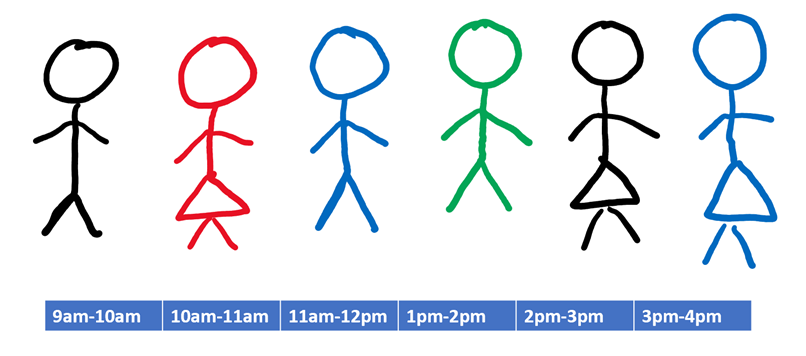
\includegraphics[keepaspectratio]{workers.png}}

}

\caption{Here is the caption text}

\end{figure}%

\subsubsection*{Approach 2 (R)}\label{approach-2-r}
\addcontentsline{toc}{subsubsection}{Approach 2 (R)}

This is a slightly more difficult approach and requires the use of R,
but it is better for ``hiding'' the alternative text.

\begin{Shaded}
\begin{Highlighting}[]
\InformationTok{\textasciigrave{}\textasciigrave{}\textasciigrave{}\{r, echo=FALSE, out.width="600px", fig.alt="Here is the alt text",}
\InformationTok{    fig.cap="Here is the image caption."\}}
\InformationTok{    knitr::include\_graphics("workers.png")}
\InformationTok{\textasciigrave{}\textasciigrave{}\textasciigrave{}}
\end{Highlighting}
\end{Shaded}

\begin{figure}[H]

{\centering 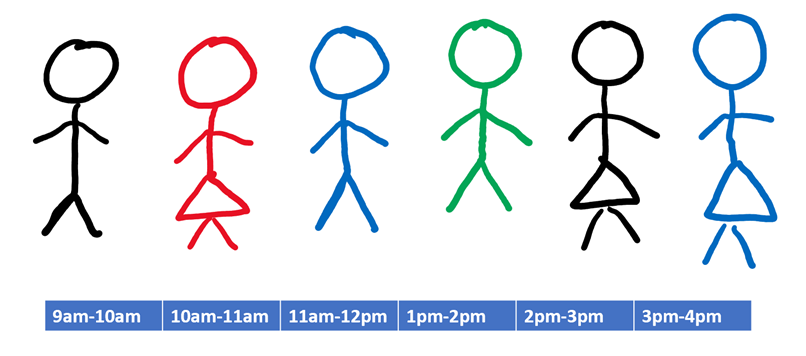
\includegraphics[width=6.25in,height=\textheight,keepaspectratio]{workers.png}

}

\caption{Here is the image caption.}

\end{figure}%

The student could view the alt text by right clicking on the image and
selecting ``Inspect Element'', or by using suitable assistive
technology.

This is the preferred approach since we can distinguish between image
captions and alt text. Also, we benefit from R's automatic numbering of
figures in their captions.

\subsection{Generating Images Using R (or
Python)}\label{generating-images-using-r-or-python}

Use the following format to add R code. This adds the chunk below and
you can add in R code. Python (or other languages) can also be added by
changing the prefix to `python' and change the setting accordingly
\href{https://quarto.org/docs/computations/python.html}{(python
setting)}.

\begin{Shaded}
\begin{Highlighting}[]
\NormalTok{::: \{.example name="Create Image Using R"\}}
\InformationTok{\textasciigrave{}\textasciigrave{}\textasciigrave{}\{r,fig.alt="A graph that shows...", fig.cap="A graph demonstrating..."\}}
\InformationTok{x\textless{}{-}rnorm(100,mean=4,sd=2)}
\InformationTok{y\textless{}{-}x\^{}\{2\}}
\InformationTok{plot(x,y,lwd=4,main="Mock plot")}
\InformationTok{\textasciigrave{}\textasciigrave{}\textasciigrave{}}
\NormalTok{:::}
\end{Highlighting}
\end{Shaded}

\begin{Shaded}
\begin{Highlighting}[]
\NormalTok{x}\OtherTok{\textless{}{-}}\FunctionTok{rnorm}\NormalTok{(}\DecValTok{100}\NormalTok{,}\AttributeTok{mean=}\DecValTok{4}\NormalTok{,}\AttributeTok{sd=}\DecValTok{2}\NormalTok{)}
\NormalTok{y}\OtherTok{\textless{}{-}}\NormalTok{x}\SpecialCharTok{\^{}}\NormalTok{\{}\DecValTok{2}\NormalTok{\}}
\FunctionTok{plot}\NormalTok{(x,y,}\AttributeTok{lwd=}\DecValTok{4}\NormalTok{,}\AttributeTok{main=}\StringTok{"Mock plot"}\NormalTok{)}
\end{Highlighting}
\end{Shaded}

\begin{figure}[H]

{\centering \pandocbounded{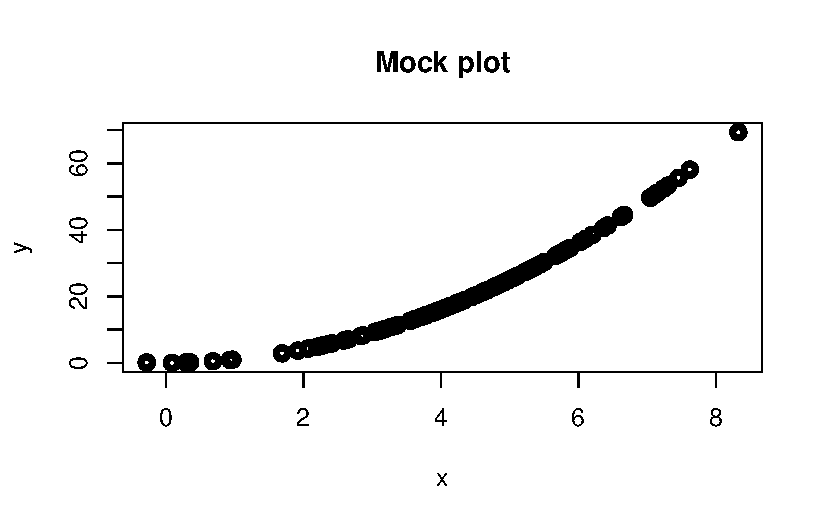
\includegraphics[keepaspectratio]{02-Part2_files/figure-pdf/unnamed-chunk-13-1.pdf}}

}

\caption{A graph demonstrating\ldots{}}

\end{figure}%

You can also hide code, so that graphs are produced without showing the
code, or you can hide output so the code is shown without the results
etc. see
\href{https://quarto.org/docs/computations/execution-options.html}{the
Quarto execution options} for more information.

The graph is produced but the code is hidden, by setting echo=FALSE.

\begin{figure}[H]

{\centering \pandocbounded{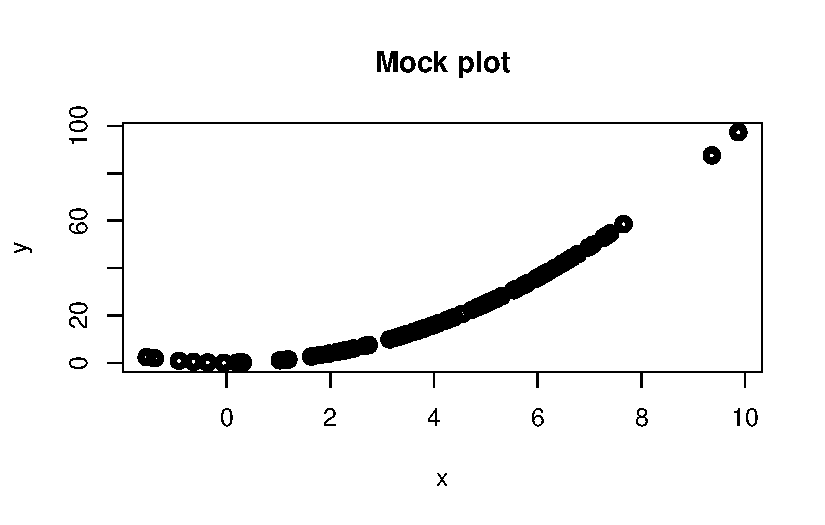
\includegraphics[keepaspectratio]{02-Part2_files/figure-pdf/unnamed-chunk-14-1.pdf}}

}

\caption{A graph demonstrating\ldots{}}

\end{figure}%

Here, the code is shown but the graph is not shown using eval=FALSE.

\begin{Shaded}
\begin{Highlighting}[]
\NormalTok{x}\OtherTok{\textless{}{-}}\FunctionTok{rnorm}\NormalTok{(}\DecValTok{100}\NormalTok{,}\AttributeTok{mean=}\DecValTok{4}\NormalTok{,}\AttributeTok{sd=}\DecValTok{2}\NormalTok{)}
\NormalTok{y}\OtherTok{\textless{}{-}}\NormalTok{x}\SpecialCharTok{\^{}}\NormalTok{\{}\DecValTok{2}\NormalTok{\}}
\FunctionTok{plot}\NormalTok{(x,y,}\AttributeTok{lwd=}\DecValTok{4}\NormalTok{,}\AttributeTok{main=}\StringTok{"Mock plot"}\NormalTok{)}
\end{Highlighting}
\end{Shaded}

\section{Environments}\label{environments}

Quarto Bookdown has several built-in environments, such as Theorem,
Example, etc to help organise your notes.

\subsection{Numbered Environments}\label{numbered-environments}

The following environments have an automatic numbering system and so can
be cross-referenced.

\begin{longtable}[]{@{}lll@{}}
\caption{Numbered Environments in Quarto
Bookdown}\label{tbl-numEnvs}\tabularnewline
\toprule\noalign{}
Environment & Printed Name & Label Prefix \\
\midrule\noalign{}
\endfirsthead
\toprule\noalign{}
Environment & Printed Name & Label Prefix \\
\midrule\noalign{}
\endhead
\bottomrule\noalign{}
\endlastfoot
theorem & Theorem & thm \\
lemma & Lemma & lem \\
corollary & Corollary & cor \\
proposition & Proposition & prp \\
conjecture & Conjecture & cnj \\
definition & Definition & def \\
example & Example & exm \\
exercise & Exercise & exr \\
hypothesis & Hypothesis & hyp \\
\end{longtable}

This green box is the \texttt{example} environment. To invoke the
\texttt{example} environment, use the syntax

\begin{Shaded}
\begin{Highlighting}[]
\NormalTok{::: \{.example name="Example Name"\}}
\NormalTok{\textless{}br\textgreater{}}
\NormalTok{Example text...}
\NormalTok{:::}
\end{Highlighting}
\end{Shaded}

If you do not wish to name your example, then write

\begin{Shaded}
\begin{Highlighting}[]
\NormalTok{:::example}
\NormalTok{\textless{}br\textgreater{}}
\NormalTok{Example text...}
\NormalTok{:::}
\end{Highlighting}
\end{Shaded}

The \texttt{\textless{}br\textgreater{}} tag is used to start the
example text on a new line.

\subsubsection*{Cross Referencing
Environments}\label{cross-referencing-environments}
\addcontentsline{toc}{subsubsection}{Cross Referencing Environments}

Numbered environments are cross referenced in a similar way to equations
(see \hyperref[mathematics]{Section 2.3}).

\begin{Shaded}
\begin{Highlighting}[]
\NormalTok{::: \{.theorem \#thm{-}pyth name="Pythagoras\textquotesingle{} Theorem"\}}
\NormalTok{\textless{}br\textgreater{}}
\NormalTok{For a right{-}angled triangle, if $c$ denotes the length of the hypotenuse}
\NormalTok{and $a$ and $b$ denote the lengths of the other two sides, we have}
\NormalTok{$$a\^{}2 + b\^{}2 = c\^{}2.$$}
\NormalTok{:::}
  
\NormalTok{We use Pythagoras\textquotesingle{} @thm{-}pyth to find the length of the missing side.}
\end{Highlighting}
\end{Shaded}

\begin{theorem}[Pythagoras'
Theorem]\protect\hypertarget{thm-pyth}{}\label{thm-pyth}

For a right-angled triangle, if \(c\) denotes the length of the
hypotenuse and \(a\) and \(b\) denote the lengths of the other two
sides, we have \[a^2 + b^2 = c^2.\]

\end{theorem}

We use Pythagoras' Theorem~\ref{thm-pyth} to find the length of the
missing side.

The syntax for referencing environments is
\texttt{@\textless{}prefix\textgreater{}-\textless{}label\textgreater{}}.
Refer to Table~\ref{tbl-numEnvs} for the prefix corresponding to each
environment type. And please note that you do not have to include the
\texttt{prefix} in the sentence.

Specially for tables, the following format is required.

\begin{Shaded}
\begin{Highlighting}[]

\FunctionTok{\#\#\# Unnumbered Environments}

\NormalTok{|Environment| Printed Name |}
\NormalTok{|:{-}{-}{-}{-}{-}{-}|:{-}{-}{-}{-}{-}{-}{-}|}
\NormalTok{|proof | Proof |}
\NormalTok{|remark | Remark|}
\NormalTok{|note | Note|}
\NormalTok{|tip | Tip|}
\NormalTok{|activity| Activity|}
\NormalTok{|discussion| Discussion|}
\NormalTok{|solution| Solution|}

\NormalTok{: Other Environments in Quarto Bookdown \{\#tbl{-}otherEnv\}}
\end{Highlighting}
\end{Shaded}

\subsection{Unnumbered Environments}\label{unnumbered-environments}

\begin{longtable}[]{@{}ll@{}}
\caption{Other Environments in Quarto
Bookdown}\label{tbl-otherEnv}\tabularnewline
\toprule\noalign{}
Environment & Printed Name \\
\midrule\noalign{}
\endfirsthead
\toprule\noalign{}
Environment & Printed Name \\
\midrule\noalign{}
\endhead
\bottomrule\noalign{}
\endlastfoot
proof & Proof \\
remark & Remark \\
note & Note \\
tip & Tip \\
activity & Activity \\
discussion & Discussion \\
solution & Solution \\
\end{longtable}

We have written a custom template for use in The School of Mathematical
Sciences with a specific colour scheme and some additional environments.
The code for the School Template is in \texttt{style.css}.

If you want to make adjustments to the colour scheme, or add your own
custom environments, then either edit your local copy of
\texttt{style.css} and \texttt{themes} folder, or (if you're not
familiar with CSS) contact
\href{mailto:lisa.mott@nottingham.ac.uk}{Lisa} to request a
change/update.

\bookmarksetup{startatroot}

\chapter{Interactivity}\label{interactivity}

The great thing with using HTML is that you can make your notes as
interactive as you like. This section shows you a few ways of
introducing interactivity to your notes, but the possibilities are
endless.

\section{Reveal Hidden Text}\label{reveal-hidden-text}

You can hide and unhide some text (e.g.~hints or optional solutions) as
in the following example.

Use the ``\textless details\textgreater{}'' and
``\textless summary\textgreater{}'' html tags to hide and reveal text
interactively.

\begin{Shaded}
\begin{Highlighting}[]
\DataTypeTok{\textless{}}\KeywordTok{details}\DataTypeTok{\textgreater{}}
  \DataTypeTok{\textless{}}\KeywordTok{summary}\DataTypeTok{\textgreater{}}\NormalTok{click to unhide}\DataTypeTok{\textless{}/}\KeywordTok{summary}\DataTypeTok{\textgreater{}}
\NormalTok{  Here is some hidden text.}
\DataTypeTok{\textless{}/}\KeywordTok{details}\DataTypeTok{\textgreater{}}
\end{Highlighting}
\end{Shaded}

click to unhide.

This is the text/image etc. that I want to hide.

\(a+b\)

\begin{Shaded}
\begin{Highlighting}[]
\NormalTok{x}\OtherTok{\textless{}{-}}\FunctionTok{rnorm}\NormalTok{(}\DecValTok{100}\NormalTok{,}\AttributeTok{mean=}\DecValTok{4}\NormalTok{,}\AttributeTok{sd=}\DecValTok{2}\NormalTok{)}
\NormalTok{y}\OtherTok{\textless{}{-}}\NormalTok{x}\SpecialCharTok{\^{}}\NormalTok{\{}\DecValTok{2}\NormalTok{\}}
\FunctionTok{plot}\NormalTok{(x,y,}\AttributeTok{lwd=}\DecValTok{4}\NormalTok{,}\AttributeTok{main=}\StringTok{"Mock plot"}\NormalTok{)}
\end{Highlighting}
\end{Shaded}

\begin{figure}[H]

{\centering \pandocbounded{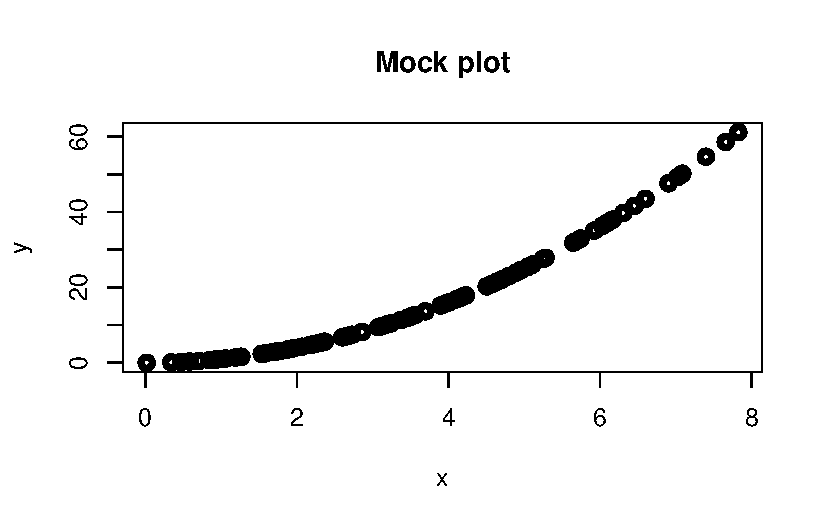
\includegraphics[keepaspectratio]{03-Part3_files/figure-pdf/unnamed-chunk-2-1.pdf}}

}

\caption{A graph demonstrating\ldots{}}

\end{figure}%

\section{Embedded Video}\label{embedded-video}

Please watch the video below to see how we have embedded this video from
mediaspace.

If the link does not work then please use
\href{https://mediaspace.nottingham.ac.uk/media/How+to+get+the+embed+links/1_824b1mfn}{this
alternative link.}

\textbf{How to use the template - Another video example}

Note to use all of this you will need some IDE and R to be installed on
your machine. Then you just need to open the project in your IDE.

Then just create a new .qmd file to add a new chapter and add it into
\texttt{\_quarto.yaml} for the order you want that chapter to appear.

A video below shows what to do in more detail. If the video does not
work then please use
\href{https://mediaspace.nottingham.ac.uk/media/How+to+use+the+template/1_brjfqb44}{this
alternative link.}

\section{Quizzes}\label{quizzes}

\subsection{Xerte}\label{xerte}

For Xerte, just paste the embed code. Example below. Note, if you have
your settings on Xerte so that the file can only be viewed from Moodle,
then the Xerte file will only show if the Rbookdown file is uploaded to
Moodle.

If the interactive slides above do not work then please access them
using \href{https://www.nottingham.ac.uk/toolkits/play_25775}{this
link.}

\subsection{Itempool}\label{itempool}

Here we use r commands to add in a URL.

\subsection{Microsoft Forms}\label{microsoft-forms}

This one has been used by copying and pasting the embed code from the
microsoft form share settings.

\bookmarksetup{startatroot}

\chapter{Adding colour}\label{adding-colour}

This is an advanced feature for bookdown and is not suitable for
beginners.

It is quite easy to use HTML to add {colour to text.} However when you
change the theme to night you will not be able to see the colour.

To display content only in light mode, use the .light-content CSS class;
to display content only in dark mode, use the .dark-content class.

Usually you should provide light and dark content in the same place and
at the same size, so that page layout is unaffected when switching
between modes.

For example, the paragraph produced by the following code will contain
different text in light and dark mode:

\begin{verbatim}
::: {.light-content}
<span style="color:blue">This text will be shown in light mode.</span>
:::

::: {.dark-content}
<span style="color:green">This text will be shown in dark mode.</span>
:::
\end{verbatim}

{This text will be shown in light mode.}

{This text will be shown in dark mode.}

\section{Adding colour to maths
output}\label{adding-colour-to-maths-output}

This is even more complicated and uses the style file. We have set three
default colours for blue, red and green that meet accessibility
requirements in the three different themes.

\[
g(\color{blue}{x-1}) = 3(\color{red}{x-1}) + 1 = \color{green}{3x} - 3 + 1 = 3x-2.
\]

\section{New box types}\label{new-box-types}

We have added some new box types to the template.

Watch out for this common mistake!

Here is a key point.


\backmatter


\end{document}
